\chapter{Grundlagen}

In diesem Kapitel wird das Wissen vermittelt, welches benötigt wird um zu Verstehen, wie \acp{NNUE} im Rahmen von Schachcomputern funktionieren. Zuerst wird die Evaluation, wie sie in herkömmlichen Schachcomputern funktioniert erklärt, auch \ac{HCE} genannt. Weiterhin werden die grundlegenden Bestandteile, die für überwacht lernende \acp{FNN} von Bedeutung sind, eingegangen. Zuletzt erläutert was \ac{SIMD} ist und wie diese Vektoroperationen in C/C++ verwendet werden können.

\section{Hand-crafted Evaluation}
\label{chap:HCE}

Es ist wichtig zu wissen wie die \ac{HCE} eines Schachcomputers funktioniert, da sie nicht nur die Variante die in jedem starken Schachcomputer vor 2017 eingesetzt wurde, sondern auch heute noch in Kombination mit \ac{NNUE} eingesetzt wird. Bei \ac{NNUE} Schachcomputern wird sie oft in Kombination mit der \ac{NN} evaluation genutzt, weil sie besser in extremen Stellungen funktioniert. Besitzt beispielsweise Weiß in einer Position eine Dame mehr, muss nicht die teurere Berechnung des \acp{NNUE} durchgeführt werden, um zu entscheiden, dass Weiß im Vorteil ist.

Die \ac{HCE} einer Schachposition ist eine heuristische Methode der Position einen numerischen Wert zuzuordnen. Vor der Verbreitung von \acp{NN}, war \ac{HCE} die einzige Form der Positions-Evaluation. Gäbe es unendliche Ressourcen könnten aus jeder Position alle mögliche Zugfolgen per Brute-Force bestimmen und der Positionen einer der drei Werte: -1 (Verlust), 0 (remis), 1 (Gewinn) geben. In der Realität ist es nicht möglich den exakten Wert der Stellung zu kennen, deshalb wird in der \ac{HCE} versucht anhand von Menschen festgelegten Kriterien einen Wert der Position zuzuordnen. Die so gewonnene Bewertung wird in der Zugsuche verwendet, um den besten Zug, abhängig von den per Hand gewählten Kriterien, zu finden. Die Evaluation wird aus Sicht der Seite, die gerade am Zug ist angegeben. Das ist wichtig für den verwendeten Suchalgorithmus (Alpha-Beta-Suche) \cite{Slagle1969}.

Die \ac{HCE} eines Schachcomputers ähnelt in einigen Aspekten mehr eine Philosophie als eine Funktion. Schach ist ein Spiel, das es seit über 1000 Jahren gibt. In dieser Zeit haben Menschen regeln überlegt, um besser Schach zu spielen. All diese Regeln in die Evaluationsfunktion zu integrieren, ist nicht ratsam. Es ist ein Abwägen zwischen Wissen und Geschwindigkeit. Je mehr regeln dem Computer geben werden, umso weniger Zeit weit kann er Vorausschauen.

Wenn ein Mensch Schach spielen lernt, ist der Wert der Figuren eines der ersten Erkenntnisse. Das ist ebenfalls der wichtigste Faktor für einen Schachcomputer \cite{Levy1988}. Die Angabe der Materialwertung wird bei Computern als Centipawn angegeben, um so mehr Spielraum für feingranulare Faktoren zu lassen. Figuren werden ebenfalls anhand ihrer Position bewertet. Dafür gibt es sogenannte Piece Square Tables, die jeder Figur abhängig von ihrer Position einen Wert zuordnen. Beispielsweise ist ein Springer am Rand des Brettes deutlich weniger Wert als einer im Zentrum, auch bekannt als \enquote{ein Springer am Rand bringt Kummer und Schand}. Weitere nennenswerte Aspekte der \ac{HCE} sind

% weitere evlauations aspekte

% erklären warum verschiedene Spielphasen eine rolle spielen

% vl noch was zu NNs

\section{Neuronale Netze}

\begin{figure}
  \centering
  % inspired by: https://tex.stackexchange.com/questions/153957/drawing-neural-network-with-tikz
  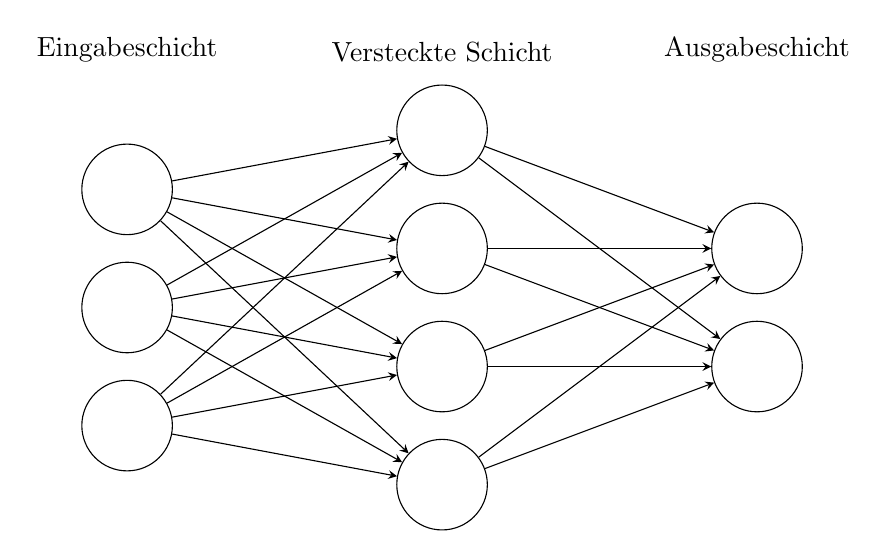
\begin{tikzpicture}[x=2cm, y=1.5cm, >=stealth]
    \tikzstyle{neuron}=[draw,shape=circle,minimum size=1.15cm]
    % draw nerons
    \foreach \m/\l [count=\y] in {1,2,3}
    \node [neuron] (input-\m) at (0,2-\y) {};

    \foreach \m [count=\y] in {1,2,3,4}
    \node [neuron] (hidden-\m) at (2,2.5-\y) {};

    \foreach \m [count=\y] in {1,2}
    \node [neuron] (output-\m) at (4,1.5-\y) {};
    % draw lines  
    \foreach \i in {1,2,3}
    \foreach \j in {1,2,3,4}
    \draw [->] (input-\i) -- (hidden-\j);

    \foreach \i in {1,2,3,4}
    \foreach \j in {1,2}
    \draw [->] (hidden-\i) -- (output-\j);

    \foreach \l [count=\x from 0] in {Eingabeschicht, Versteckte Schicht, Ausgabeschicht}
    \node [align=center, above] at (\x*2,2) {\l};
  \end{tikzpicture}
  \caption{Ein einfaches \acl{NN}}
  \label{fig:beispiel-nn}
\end{figure}

\Acp{KNN} oder einfach \acp{NN} genannt, sind Computer Systeme, die dem biologischen Vorbild des Gehirns nachempfunden sind. Analog zu seinem biologischen Vorbild besteht ein \ac{NN} aus Neuronen die miteinander Vernetzt sind. Jedes Neuron reagiert auf eingehende Signal mit einer bestimmten Reaktion. Diese Reaktion kann sich durch neu gewonnene Erfahrungen anpassen, das ermöglicht es zu lernen und zukünftig besser zu reagieren.

% erklären wie der generelle aufbau ist
In Abbildung \autoref{fig:beispiel-nn} ist ein einfaches \acl{NN} zu sehen. Es besteht aus drei Schichten. Die erste Schicht, die Eingabeschicht, nimmt Eingabedaten entgegen. Eingabedaten können ganz unterschiedliche daten Repräsentieren, ist der Eingabedatensatz beispielsweise ein 100×100 Schwarzweiß-Bild, bestände die Eingabeschicht aus 1000 Neuronen die pro Neuron den Zustand eines Pixels (0 = weiß, 1 = Schwarz) des Bildes gefüttert bekommen. Die zweite Schicht heißt versteckte Schicht, weil von außen nur die Eingabedaten und das Ergebnis sichtbar ist. Sie empfängt die Informationen der Eingabeschicht, gewichtet sie und gibt sie an der Ausgabeschicht weiter. Die versteckte Schicht kann aus mehreren Schichten bestehen. Ein \ac{NN} mit mehreren versteckten Schichten heißt \ac{DNN}. Die letzte Sicht, die Ausgabeschicht, spiegelt das Ergebnis des \acp{NN} dar. Ein Netz, das versucht Bilder zwischen Hunden und Katzen zu unterscheiden kann zwei Ausgabeneuronen enthalten, eins für die Wahrscheinlichkeit das auf dem gegebenen Bild ein Hund ist und eins für die Wahrscheinlichkeit das es eine Katze ist. Ein \ac{NN} kann auch nur ein Ausgabeneuron besitzen, wie \zb{} bei der Evaluation einer Schachposition nötig ist. Die Verbindungen der einzelnen Neuronen stellen deren Zusammenhang dar. Wie stark dieser Abhängigkeit ist, wird durch Gewichte definiert \cite[S. 2--7]{krawczak2013multilayer}.
% auswahl der Input daten spalten gibt an wieviele input neuronen es gibt, die anzal der hidden neuronen ist "egal" je mehr -> desto besser kann das neuronale netz lernen kinda, output neuronen gibt die anzahl der klassifikationen an, kann auch nur eins sein (regession)

Es gibt verschiedene Modelle \aclp{NN}, für diese Thesis sind lediglich \acp{FNN} relevant. \acp{FNN} basieren auf dem von \citeauthor{rosenblatt1958perceptron} \cite{rosenblatt1958perceptron} beschriebenen mehrlagigen Perzeptron. Das \ac{FNN} zeichnet sich durch seinen Zyklen freien Aufbau aus. Der Datenfluss führt immer von der Eingabeschicht zu Ausgabeschicht. Das \ac{FNN} gilt als die einfachste Netzwerkarchitektur \cite{Schmidhuber2015}.

In den folgenden Unterabschnitten wird Grundlegend auf die Einzelteile neuronaler Netze eingegangen. To-do.

\subsection{Das Neuron}

\begin{figure}
  \centering
  % inspired by: https://davidstutz.de/illustrating-convolutional-neural-networks-in-latex-with-tikz/
  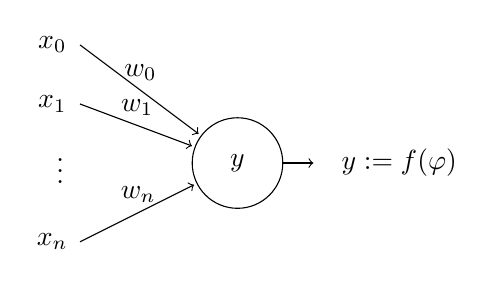
\begin{tikzpicture}[shorten >=1pt,->]
    \tikzstyle{unit}=[draw,shape=circle,minimum size=1.15cm]

    \node[unit](p) at (2,1){$y$};
    \node(dots) at (-0.25,1){\vdots};

    \draw (0,2.5) node[xshift=-10]{$x_0$} -- node [midway,above] {$w_{0}$} (p);
    \draw (0,1.75) node[xshift=-10]{$x_1$} -- node [midway,above] {$w_{1}$} (p);
    \draw (0,0) node[xshift=-10]{$x_n$} -- node [midway,above] {$w_{n}$} (p);
    \draw (p) -- (3,1) node[xshift=30]{$y := f(\varphi)$};
  \end{tikzpicture}
  \caption{Ein einzelnes Neuron mit seinen eingabe- und Ausgabekomponenten}
  \label{fig:neuron}
\end{figure}

% neuronen wie sie im nerfen systems eines menschen vorhanden sind
Das Neuron ist der elementare Bestandteil eines \acp{NN}. Es wurde \citeyear{McCulloch1943} von \citeauthor{McCulloch1943} \cite{McCulloch1943} eingeführt. Neuronen sind in einem \ac{NN} mit anderen Neuronen verbunden und bilden so beliebig komplexe Funktionen ab. In \autoref{fig:neuron} ist ein einzelnes Neuron zu sehen. Die Eingänge $x_{0}$ bis $x_{n}$, werden mit den Gewichten $w_{0}$ bis $w_{n}$ multipliziert und aufsummiert und mit der Aktivierungsfunktion $f(\varphi)$ wird die Ausgabe des Neurons. Für gewöhnlich ist immer $x_{0}=1$, was ihn zu dem Bias des Neurons mit $w_{0}=b$ macht. Das bedeutet, dass es nur $n$ tatsächliche Eingabewerte gibt: von $x_{1}$ bis $x_{n}$. Konkret lässt sich die Aktivität eines Neurons mit der \autoref{equation:NeuronActivation} und die Ausgabe $y$ mit \autoref{equation:NeuronOutput} bestimmen:

\begin{equation}
  f(\varphi) = \varphi(\sum_{i=0}^{n}w_{j}x_{j})
  \label{equation:NeuronActivation}
\end{equation}

\begin{equation}
  y = f(\varphi)
  \label{equation:NeuronOutput}
\end{equation}

\begin{figure}
  \centering
  \begin{subfigure}{.5\textwidth}
    \centering
    \resizebox{.9\textwidth}{!}{%
      \begin{tikzpicture}[declare function={sigma(\x)=1/(1+exp(-\x));}]
        \begin{axis}%
          [
            grid=none,
            xmin=-6,
            xmax=6,
            axis x line=bottom,
            ytick={0,.5,1},
            ymax=1,
            axis y line=middle,
            samples=100,
            domain=-6:6,
            legend style={at={(1,0.9)}}
          ]
          \addplot[blue,mark=none]   (x,{sigma(x)});
        \end{axis}
      \end{tikzpicture}
    }
    \caption{Standardsigmoide Aktivierungsfunktion}
    \label{fig:sigmoid}
  \end{subfigure}%
  \begin{subfigure}{.5\textwidth}
    \centering
    \resizebox{.9\textwidth}{!}{%
      \begin{tikzpicture}[declare function={relu(\x)=max(0,\x);}]
        \begin{axis}%
          [
            grid=none,
            xmin=-3,
            xmax=3,
            axis x line=bottom,
            ytick={0,1,2,3},
            ymax=3,
            axis y line=middle,
            samples=1000,
            domain=-3:3,
            legend style={at={(1,0.9)}}
          ]
          \addplot[blue,mark=none]   (x,{relu(x)});
        \end{axis}
      \end{tikzpicture}
    }
    \caption{Rectified Linear Aktivierungsfunktion}
    \label{fig:ClippedRelu}
  \end{subfigure}
  \caption{Beispiele für Aktivierungsfunktionen}
  \label{fig:activationfunction}
\end{figure}

Die Aktivierungsfunktion, oder auch Transferfunktion, eines Neurons kann linear oder nicht linear sein. Ist die Transferfunktion linear, ergibt ein mehrschichtiges \ac{NN} keinen Sinn, da sie zu einer Schicht vereinfacht werden können. Lineare \acp{NN} sind nicht in der Lage, nicht lineare Probleme zu lösten \cite{minsky1969perceptron}. Nicht lineare Transferfunktionen sind interessanter, da sie für nicht lineare Probleme antworten liefern können. In \autoref{fig:activationfunction} sind zwei Aktivierungsfunktionen zu sehen. In \autoref{fig:sigmoid}
% activation functions: linear vs non linear -> linear functions sorgen dafür das nur ein hidden layer sinnvoll ist, mehrere hidden layer mit linearen Aktivierungs Funktionen geben keinen sinn, da sie zu einer Schicht vereinfacht werden können. Deshalb sind nicht-lineare Transferfunktionen interessant, sie ermöglichen es komplexere Funktionen zu lernen

% eingehen auf Clipped relu und sigmoid aktivation functions
% mathe matische grundlage für das neuron und neuronale netz
\ac{ReLU}

\subsection{Backpropagation}
% viel muss man davon nicht kennen, da pytorch das übernimmt (automatic through automatic differentiation)
Als Backpropagation wird das Verfahren der Fehlerrückführung beschrieben. Es gehört zu der Familie der überwachten Lernverfahren

% Die delta lern regel

% the forward pass gives you the error and the backpropagation computes the gradiants and based on the gradiants the optimization algorithm ajusts the weights, the learing rate is the speed at witch changes occure

% \subsection{Convolutional Neural Networks}
% kann vl entfernt werden (schau am ende ob man es noch braucht (seiten))
% nur ein kurzer exkurs da es in andern neuronalen netzen für schach computer verwendet wird


\subsection{Loss Functions}

\subsection{Optimierer}

% versucht probleme der backpropagation zu mitigieren
% exemplarisch auf den Adadelta optimirer eingehen, da der in dieser arbeit verwendet wurde

\subsection{Quantisierung}

Quantisierung ist ein Signalverarbeitungsverfahren, bei welchem Eingabewerte auf eine vorher festgelegte kleinere Menge von Ausgabewerten abgebildet wird. Ein simples Beispiel für Quantisierung ist das Abbilden von rationalen Zahlen auf ganze Zahlen, hierfür müssen die rationalen Zahlen zu der nächsten ganzen Zahl gerundet werden. Im Bereich der Informatik werden für Gleitkomma Eingabewerte oft Festkommazahlen oder Ganzzahlen als Ausgabewerte gewählt \cite{Gysel2016}. Egal wie und welche die Quantisierung stattfindet, das Ziel ist es weniger Speicherkapazität und weniger Berechnungszeit zu benötigen mit minimalen Präzisionsverlust. Welches Quantisierungsschema verwendet wird, hängt von dem Anwendungsfall ab und kann nicht allgemein bestimmt werden. Es ist immer ein abwägen von Leistung und Präzision.

Dieses Verfahren eignet sich gut für Anwendungsgebiete mit wenig Speicher- und Rechenkapazität, wie beispielsweise der Einsatz von \acp{NN} bei Mobilgeräten \cite{MaQuantization2019, Gysel2016}. Der Grund dafür ist zweierlei. Erstens sorgt Quantisierung dafür, dass weniger Platz im cache der CPU gebraucht wird, wodurch weniger Schreib- und Lesezugriffe ausgeführt werden und somit die Berechnung schneller ist. Zweitens ermöglicht die Abbildung auf kleinere Datentypen einen Performance-Gewinn, durch die effizientere Verwendung von Prozessor internen Recheneinheiten die beispielsweise \ac{SIMD} unterstützen. Zudem ermöglicht die Abbildung auf Ganzzahl Typen die Nutzung von CPU internen Ganzzahl-Recheneinheiten, die effizienter als die Gleitkommazahl äquivalente Funktionieren, falls überhaupt vorhanden \cite{Jacob2017}.

Das Problem der Quantisierung ist das Einbauen von \enquote{Fehlern}. Bei \acp{NN} wird oft von Fehler-Kumulierung gesprochen, da bei der Aktivierung eines \acp{NN} in jedem Quantisierten Neuron der Fehler wächst \cite{Park2018}.
% es muss immer für jeden einzelnen anwendungs fall überlegt werden ob es sich lohnt, für nnue 

\section{Training}

\section{SIMD}

Der Begriff \ac{SIMD} kommt von der flynnschen Klassifikation, die Rechnerarchitekturen in vier gebiete aufteilt \cite{Flynn1972}. Die Aufteilung orientiert sich an der Anzahl vorhandener Befehls- und Datenströme. Es gibt Single und Multiple Instructions, sowie Single und Multiple Data. Die daraus entstehenden Klassen heißen: \ac{SIMD}, \ac{SISD}, \ac{MIMD} und \ac{MISD}.

In diesem Abschnitt geht es um \ac{SIMD}. \ac{SIMD} ermöglicht in einem Prozessor Befehlszyklus, eine Instruktion auf mehere Elemente eines Vektors gleichzeitig durchzuführen. Es gibt je nach Mikroprozessor-Architektur, verschiedene Erweiterungen, um \ac{SIMD} zu implementieren. In dieser Arbeit sind alle Beispiele mit dem \ac{AVX2} Befehlssatz geschrieben. Der Grund dafür ist, dass \ac{AVX2} von Modernen Intel und AMD Mikroprozessoren unterstützt werden.

% chosing what SIMD instruction set to use:
% depends on the hardware ur using, some SIMD is only present in server grade cpus
% vl arbeit raussuchen die einen vergleich zwischen den SIMD instruction sets macht und zitieren

\subsection{Memory Alignment}

\section{NNUE}

